\section{Introduction}
\label{sec:intro}

\subsection{Background}

% The class of regular languages is remarkably stable, and can either be characterized as the 
% languages recognized by either
% (a) deterministic or non-deterministic finite state automata \cite[Proposition 1.2.3, p.~7]{pin_handbook_2021},
% (b) two-way finite state automata by Shepherdson-Rabin-Scott Ttheorem
% \cite[Theorem 2, p.~198]{shepherdson_reduction_1959} \cite[Theorem 15, p.~123]{rabin_finite_1959},
% (c) rational expressions by Kleene's theorem \cite[Theorem 1.5.11, p.~34]{pin_handbook_2021},
% (d) monadic second-order logic by Trakhtenbrot-Büchi-Elgot theorem \cite[Theorem 2.2, p.~32]{bojanczyk_languages_2020}, or
% (e) finite monoids \cite[\S 1.4.2, p.~19]{pin_handbook_2021},
% and moreover, all transformations are effective.

% \diego{softer intro?}
The landscape of rationality for $k$-ary relations of finite words ($k \geq 2$) is far more complex than for languages---recall that languages can be seen as unary relations of finite words---as depicted in \Cref{fig:landscape-rationality} on page~\pageref{fig:landscape-rationality}. Perhaps the most natural class is that of \AP""rational relations"", defined as relations accepted by non-deterministic two-tape automata---an input $(u,v)$ is described by writing $u$ on the first tape and $v$ and the second tape---that can move its two heads independently, from left to right---see \cite[\S 2.1]{carton_decision_2006} for a formal definition. For instance, the suffix relation is "rational".


Our paper focuses on "synchronous relations", "aka" "automatic relations" or "regular relations", defined as the "rational relations" that can be recognized by
"synchronous automata",
a subclass of the machines described above obtained by keeping a single head that
moves synchronously from left to right, reading one pair of letters after the other; we add
padding symbols $\pad$ at the end of the shorter word---see
\Cref{fig:ex-sync-auto}.
While the suffix relation is not "synchronous", typical examples include the prefix relation,
the same-length relation, etc.
"Synchronous relations" play a central role in the
definitions of automatic structures---introduced by Hodgson \cite{hodgson_theories_1976,hodgson_direct_1982,hodgson_decidabilite_1983} and rediscovered by Khoussainov \& Nerode \cite{goos_automatic_1995}, see \cite[\S XI, pp.~627--762]{blumensath_monadic_2023}.
They also have been studied in the context of graph databases \cite[Definition 3.1, p.7 \& Theorem 6.3, p.~13]{barcelo_expressive_2012}, see \cite[\S 8, p.~17]{figueira_foundations_2021} for more context \& results on \emph{extended} conjunctive regular path queries.
% ---in short, they are algebraic models, or more generally first-order models, which can be described by "synchronous automata": while these structures can be infinite, many problems remain decidable on them \todo{addref blumensath bis}.

\begin{figure}[htb]
	\begin{center}
		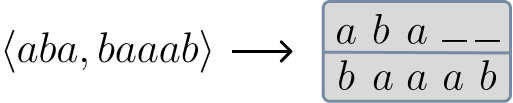
\includegraphics[width=.4\linewidth,valign=m]{fig/algebra/encoding.png}
		% \qquad
		% \begin{tikzpicture}[shorten >= 1pt, node distance = 1.8cm, on grid, baseline]
		% 	\AP\small
		% 	\node[state, initial left, accepting] (q0) {}; 
		% 	\path[->]
		% 		(q0) edge[loop right]
		% 			node {$\substack{\pair{a}{b}, \pair{\pad}{a}\\ a, b \in \Sigma}$}
		% 		(q0);
		% \end{tikzpicture}
		\qquad
		\begin{tikzpicture}[shorten >= 1pt, node distance = 1.8cm, on grid, baseline]
			\AP\small
			\node[state, initial left, accepting] (q0) {}; 
			\node[state] (q1) [right =of q0] {};
			\path[->]
				(q0) edge[loop above] node[font=\scriptsize] {$\pair{a}{a}, \pair{b}{b}, \textrm{Pad}\hspace{1.5em}$} (q0) 
				(q0) edge[bend left=20] node[above, font=\scriptsize] {$\pair{a}{b}, \pair{b}{a}$} (q1)
				(q1) edge[bend left=20] node[below, font=\scriptsize] {$\pair{a}{b}, \pair{b}{a}$} (q0)
				(q1) edge[loop above] node[font=\scriptsize] {$\hspace{1.5em}\pair{a}{a}, \pair{b}{b}, \textrm{Pad}$} (q1);
		\end{tikzpicture}
	\end{center}
	\caption{
		\label{fig:ex-sync-auto}
		Encoding a pair of words of $\Sigma^* \times \Sigma^*$ into an element of
		$(\SigmaPair)^*$ where $\SigmaPair \defeq (\Sigma \times \Sigma) \,\cup\,
		(\Sigma \times \{\pad\}) \,\cup\,
		(\{\pad\} \times \Sigma)$ (left) and 
		a deterministic complete "synchronous automaton" (right)
		over $\Sigma = \{a,b\}$ accepting the binary relation
		of pairs $(u,v)$ such that the number of $a$'s in $u_1\hdots u_k$
		and in $v_1\hdots v_k$ are the same mod $2$, where $k = \min(|u|, |v|)$. 
		$\textrm{Pad}$ denotes the set of transitions $\{\pair{a}{\pad}, \pair{b}{\pad}, \pair{\pad}{a}, \pair{\pad}{b}\}$.
	} 
\end{figure}

\begin{remark}
	All our results are described for binary relations, but can be extended to
	$k$-ary synchronous relations, see \Cref{sec:discussion}.
\end{remark}

"Synchronous relations" stand at the frontier between expressiveness and undecidability: for instance, Carton, Choffrut and Grigorieff showed that it is decidable whether an "automatic relation" is ""recognizable"" \cite[Proposition 3.9, p.~265]{carton_decision_2006}, meaning that
it can be written as a finite union of Cartesian products of regular languages.\footnote{For 
instance, the relation ``having the same length modulo $2$'' is "recognizable", since it can be 
written as $(aa)^*\times (aa)^* \cup
a(aa)^*\times a(aa)^*$.}\footnote{The problem was latter shown to be "NL"-complete and
"PSpace"-complete depending on whether the input automaton is deterministic or not
in \cite[Theorem 1, p.~3]{barcelo_monadic_2019}.}
"Synchronous relations" are effectively closed under Boolean operations---see "eg" \cite[Lemma XI.1.3, p.~627]{blumensath_monadic_2023},
and moreover, inclusion (and subsequent problems: universality, emptiness, equivalence…) is decidable for them,
by reduction to classical automata,
contrary to the equivalence problem over "rational relations"
which is undecidable \cite[Theorem 8.4, p.~81]{berstel_transductions_1979}.

However, some seemingly easy problems are undecidable: Köcher showed that
it is undecidable if the (infinite) graph defined by a "synchronous relation" is
2-colourable---\cite[Proposition 6.5, p.~43]{kocher_analyse_2014}, and Barceló, Figueira and Morvan showed that undecidability also
holds for regular 2-colourability \cite[Theorem 4.4, p.~8]{barcelo_separating_2023}.
On the other hand, one can decide
if said graph contains an infinite clique, see \cite[Corollary 5.5, p.~32]{kuske_natural_2010}:
this is a consequence of \cite[Theorem 3.20, p.~185]{Rubin_2008}. 

\subsection{Motivation}

Any "synchronous relation" can be seen as a regular language over the alphabet
$\SigmaPair \defeq (\Sigma \times \Sigma) \,\cup\,
(\Sigma \times \{\pad\}) \,\cup\, (\{\pad\} \times \Sigma)$ of pairs. On the other hand any regular language $L$ over $\SigmaPair$
produces a "synchronous relation" when intersected with the language of all
"well-formed words"---namely words where the padding symbols are consistently placed;
see \Cref{sec:preliminaries} for precise definitions. In fact, the semantics
of "synchronous automata" such as the one in \Cref{fig:ex-sync-auto} is precisely defined this way:
it is the intersection of the ``classical semantic'' of the automaton, seen as an NFA, intersected
with "well-formed words".

\begin{figure}[htbp]
	\begin{center}
		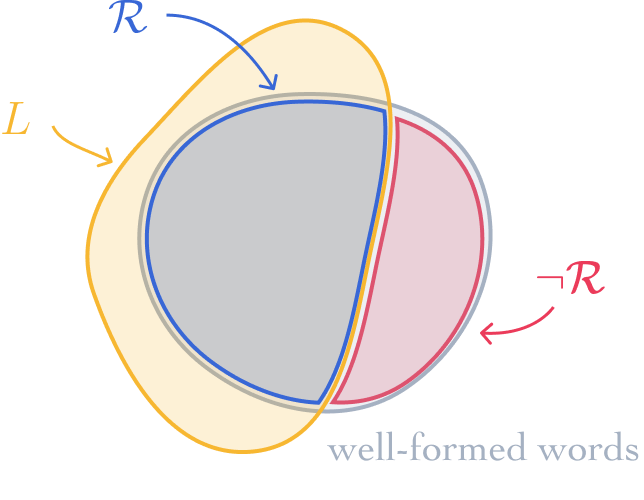
\includegraphics[width=.4\linewidth]{fig/algebra/projection.png}
	\end{center}
	\caption{
		\label{fig:projection}
		Drawing in $(\SigmaPair)^*$ of a "$\+V$-relation" $\+R$ and $\negrel\+R \defeq \{(u,v) \in \Sigma^*\times \Sigma^* \mid (u,v) \not\in \+R\}$, where $\+R$ is defined as $L \cap \WellFormed$ with $L \in \+V$.
	} 
\end{figure}

In particular, a class $\+V$ of regular languages over
$\SigmaPair$
("e.g." first-order definable languages, group languages, etc.) induces a class of so-called
"$\+V$-relations", defined as the relations over $\Sigma$ obtained as the intersection of some 
language of $\+V$ with "well-formed words", see \Cref{fig:projection}.
For instance, the relation of \Cref{fig:ex-sync-auto}
is a "$\+V$-relation" where $\+V$ is the class of all group languages---these relations can be 
alternatively described as those recognized by a deterministic complete synchronous automaton whose 
transitions functions are permutations of states.

\begin{question}
	\label{quest:V-relations}
	Given a class $\+V$ of languages, can we characterize and decide the class of "$\+V$-relations"?
\end{question}

As we will see in \Cref{ex:group-languages}, for a "relation" to be $\+V_{\SigmaPair}$
is not necessary for it to be a "$\+V$-relation".

\subsection{Contributions}

We answer positively to this question.
For this we first need to develop an algebraic theory of "synchronous relations",
which enables us to prove the lifting theorem. In short, the "lifting theorem" states that algebraic characterizations of classes of word languages can be lifted in a canonical way to algebraic characterizations of classes of word relations.

The algebraic approach usually provides more than decidability: it attaches
canonical algebras to languages/relations ("eg" monoids for languages of finite words), and often simple ways to characterize complex properties ("eg" first-order definability, see "eg" \cite[Theorem 2.6, p.~40]{bojanczyk_languages_2020}).
Our "synchronous algebras" differ from monoids in two points:
\begin{itemize}
	\item they are typed---a quite common feature in algebraic language theory, shared "eg" by $\omega$-semigroups \cite[\S 4.1, p.~91]{perrin_infinite_2004};
	% or Bojańczyk \& Walukiewicz's forest algebras \cite[\S 1.3, p.~4]{bojanczyk_forest_2008}; and
	\item they are equipped with a "dependency relation", which expresses constraints between 
	elements of different types---to our knowledge, this feature is entirely novel.\footnote{Note that algebras equipped with binary relations have been studied before, "eg" Pin's ordered 
	$\omega$-semigroups---see \cite[\S 2.4, p.~7]{pin_positive_1998}---but the constraints (here the 
	orderings) are always defined between elements of the \emph{same type}.}
\end{itemize}

Importantly, some variations are possible on the definition of "synchronous algebras":
in particular, one could get rid of the notion of "dependency relation" and 
\Cref{lem:syntactic-morphism-theorem,lem:eilenberg-sy} would still hold.
However, we show in \Cref{apdx:counterexample} that these
simplified synchronous algebras cannot characterize the property of being a "$\+V$-relation".
Therefore, the notion of "dependency" seems necessary to tackle \Cref{quest:V-relations}.
Moreover, we show that these algebras arise from a monad, but to our knowledge none of the 
meta-theorems developing algebraic language theories over monads apply to it,
see \Cref{apdx:monads} for more details.

We show that assuming that $\+V$ is a "$*$-pseudovariety of regular languages"---in short, a class of regular languages with desirable closure properties---, then the algebraic characterization of $\+V$ can be easily lifted to characterize "$\+V$-relations".

\begin{restatable*}[\reintro{Lifting theorem: Elementary Formulation}]{theorem}{liftingtheoremmonoids}
	\label{thm:lifting-theorem-monoids}
	Given a "relation" $\+R$ and a "$\ast$-pseudovariety of regular languages" $\+V$
	"corresponding@@EilenbergSg" to a "pseudovariety of monoids" $\B{V}$,
	the following are equivalent:
	\begin{enumerate}
		\item $\+R$ is a "$\+V$-relation",
		\item $\+R$ is "recognized@@sync" by a finite "synchronous algebra" $\mathbf{A}$
			whose "underlying monoids" are all in $\mathbb{V}$,
		\item all "underlying monoids" of the "syntactic synchronous algebras" $\SyntSA{\+R}$ of
			$\+R$ are in $\mathbb{V}$.
	\end{enumerate} 
\end{restatable*}

This theorem rests on a solid algebraic theory. 
First, we show the existence of "syntactic algebras@@sync" (\Cref{lem:syntactic-morphism-theorem}): 
each relation $\+R$ admits a unique canonical and minimal algebra $\SyntSA{\+R}$, which is finite 
"iff" the relation is "synchronous",
and then, we exhibit a correspondence between classes of finite algebras and classes of
synchronous relations (\Cref{lem:eilenberg-sy})---we assume suitable closure properties; these classes are called ``pseudovarieties''.
While the proof structures of \Cref{lem:syntactic-morphism-theorem,lem:eilenberg-sy} follow the classic proofs, see "eg" \cite{pin_mathematical_2022},
the "dependency relation" has to be taken into account quite carefully, leading for instance
to a surprising definition of "residuals", see \Cref{def:residuals}.

\paragraph*{Organization.} After giving preliminary results in \Cref{sec:preliminaries}, we introduce
the "synchronous algebras" in \Cref{sec:synchronous-algebras} and show the existence of
"syntactic algebras@@sync". We then proceed to prove the "lifting theorem@@monoids" for 
"$*$-pseudovarieties@@reglang" in \Cref{sec:lifting-theorem}, and after introducing "$*$-pseudovarieties of synchronous relations", we provide a more algebraic reformulation of the "lifting 
theorem@@monoidspseudovar" (\Cref{thm:lifting-theorem-monoids-pseudovarieties}).
We conclude the paper with
a short discussion in \Cref{sec:discussion}.

\subsection{Related Work}

\begin{figure}[htb]
	\centering
	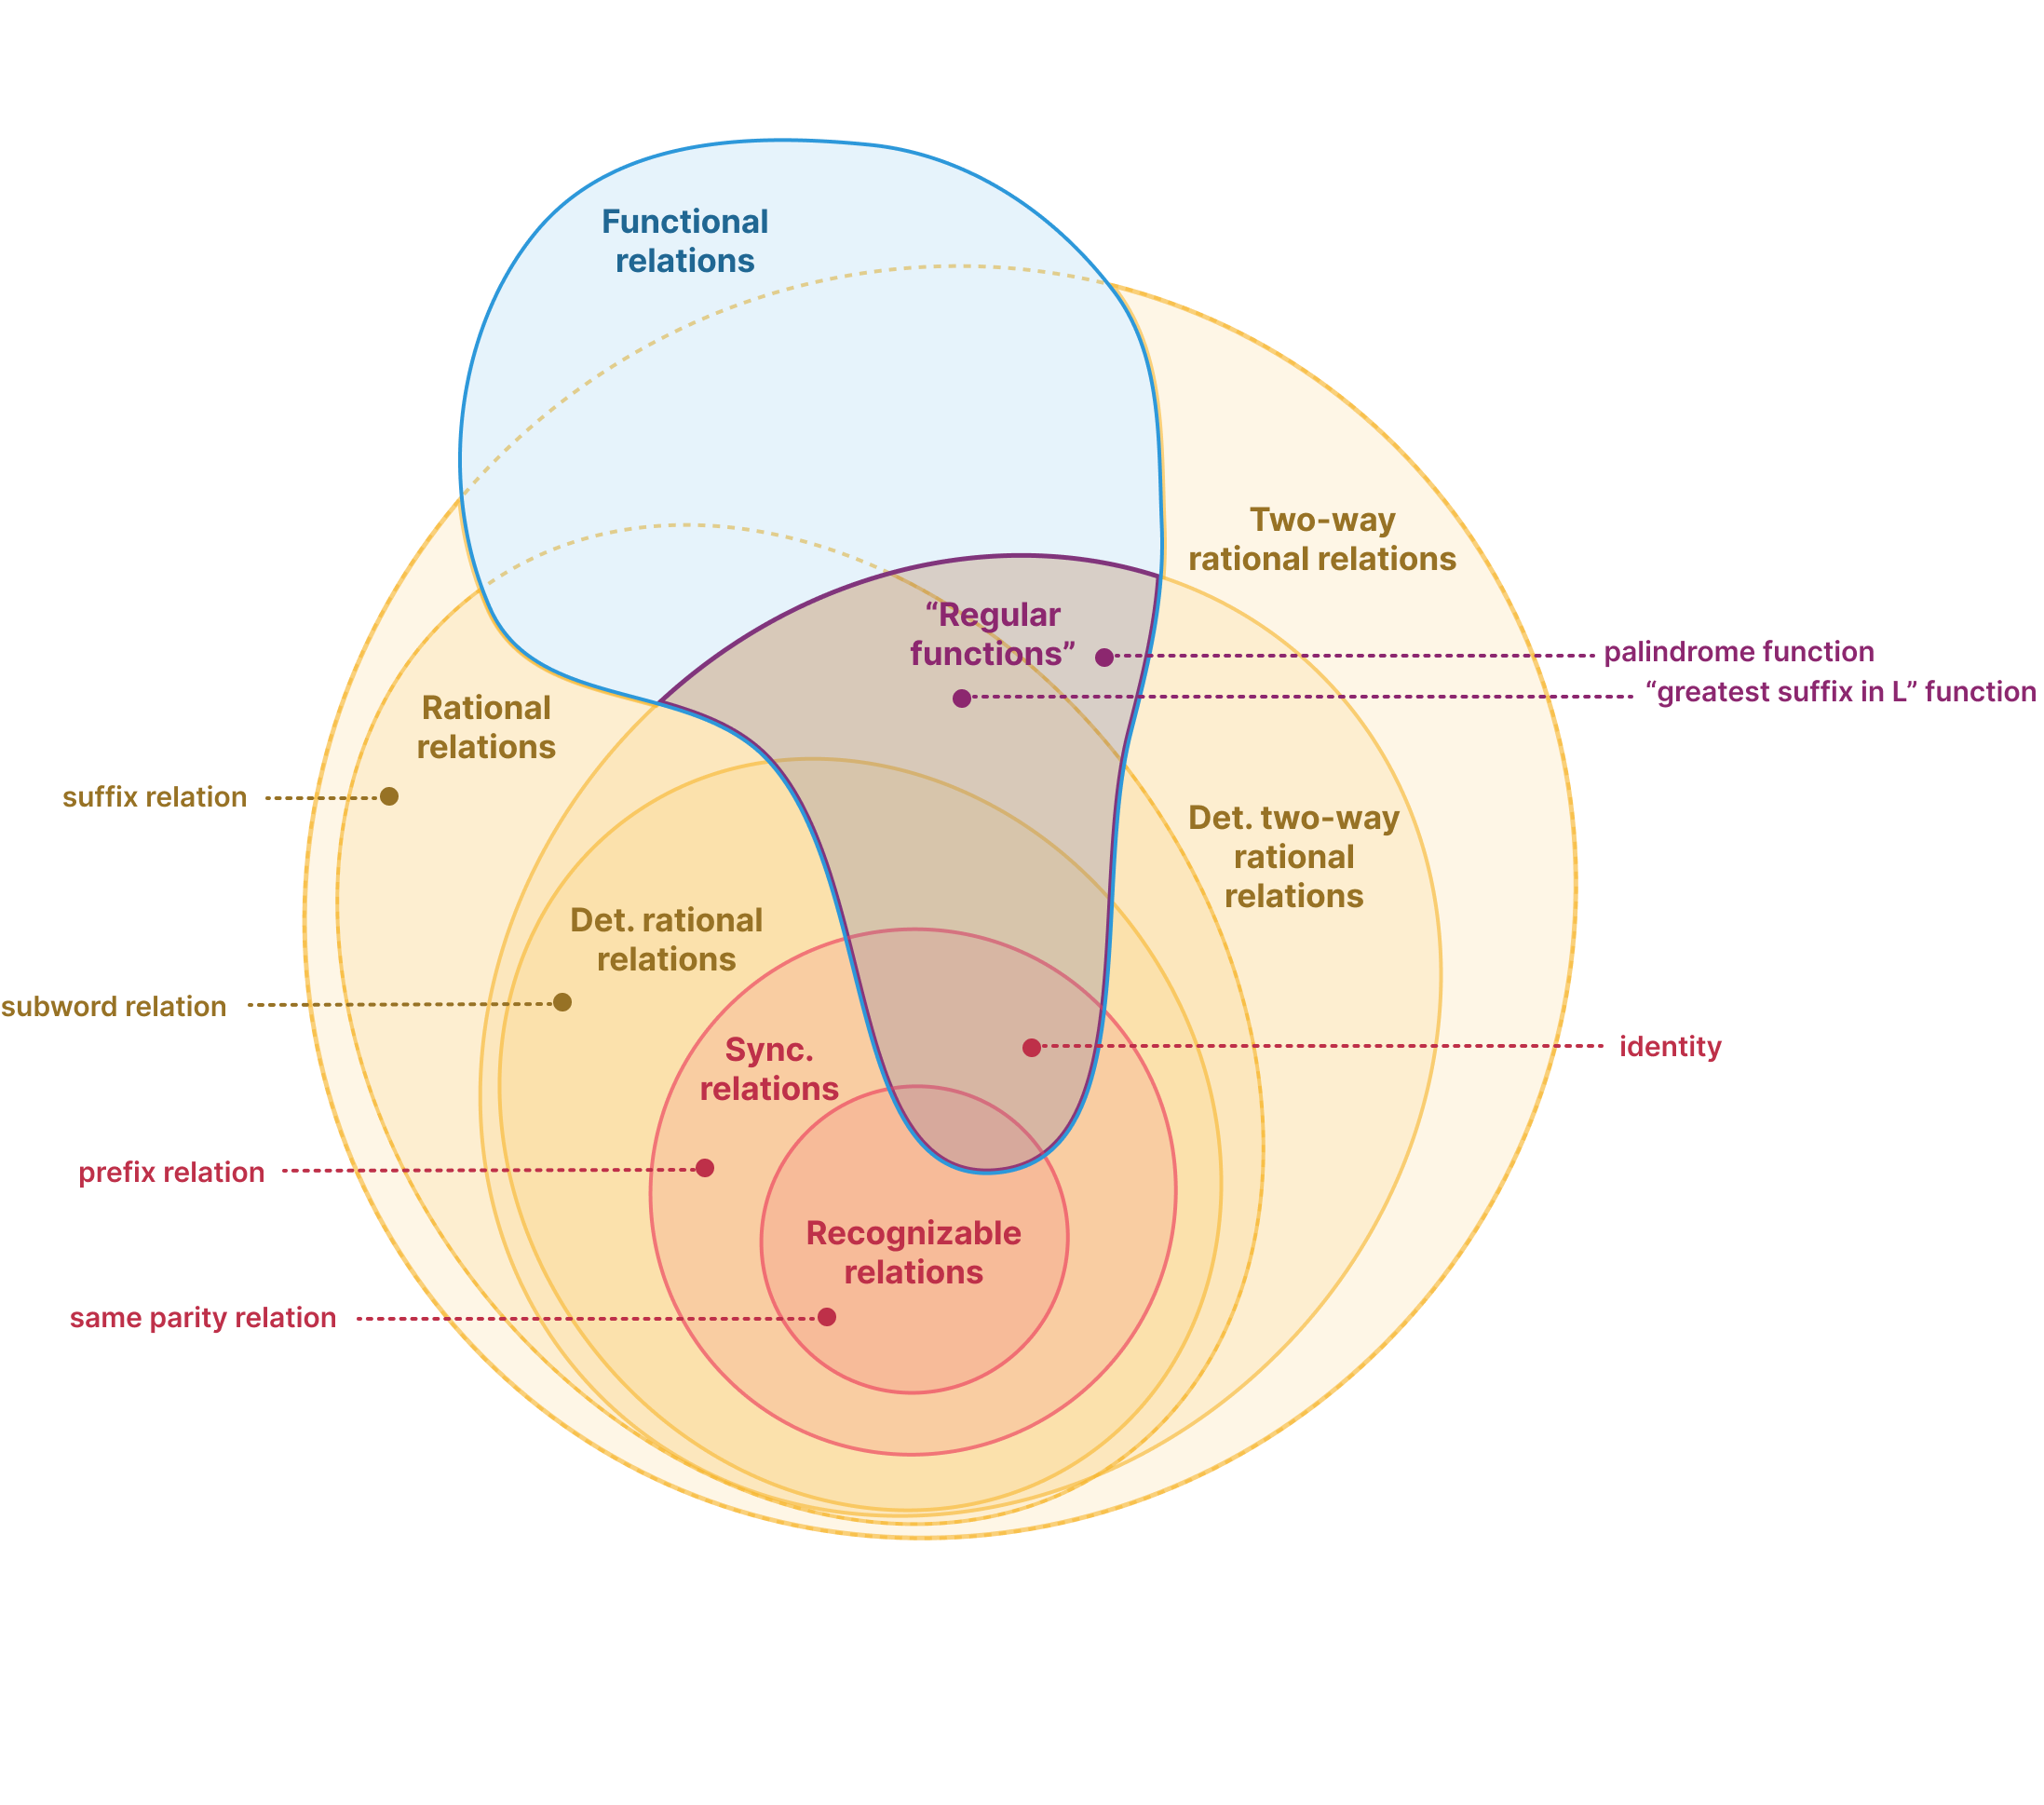
\includegraphics[width=\linewidth]{fig/algebra/landscape.png}
	\caption{
		\label{fig:landscape-rationality} The landscape of rationality for binary relations.
		Dashed regions are empty: the intersection of
		functional relations and two-way rational relations
		collapses to regular functions by
		\cite[Theorem 22, p.~243]{EH2001transduction}.
	}
\end{figure}
The algebraic framework has been extended far beyond languages of finite words: let us cite amongst other:
\begin{itemize}
	\item Reutenauer's ``algèbre associative syntactique'' for weighted languages
		\cite[Théorème I.2.1, p.~451]{reutenauer_series_1980} and their associated Eilenberg theorem \cite[Théorème III.1.1, p.~469]{reutenauer_series_1980};
	\item for languages of $\omega$-words, Wilke's algebras and $\omega$-semigroups,
		see \cite[\S II, pp.~75--131 \& \S VI, pp.~265--306]{perrin_infinite_2004};
	\item for languages over countable ordinals, Bedon defined ``$\omega_1$-semi\-groupes syntaxiques'' \cite[\S3, pp.~49--109]{bedon_langages_1998} and their Eilenberg theorem
		\cite[Theorem 22, p.~62]{bedon_eilenberg_1998};
	\item for languages over countable scattered orderings, see Rispal's ``$\Diamond$-semigroupe syntaxique'' \cite[\S 4.4, pp.~82--86]{rispal_automates_2004} and their Eilenberg theorem
		\cite[Theorem 6, p.~144]{bedon_schutzenberger_2005};
	\item more generally, for languages over countable linear orderings, see Carton, Colcombet \& Puppis' ``$\circledast$-monoids'' and ``$\circledast$-algebras''
		\cite[\S 3, p.~7]{carton_algebraic_2018};
	\item Bojańczyk \& Walukiewicz's 
		forest algebras \cite[\S 1.3, p.~4]{bojanczyk_forest_2008} \cite[\S 5, p.~159]{bojanczyk_languages_2020}
		dealing with tree languages;
	\item Engelfriet's hyperedge replacement algebras for graph languages
		\cite[\S 2.3, p.~100]{courcelle_graph_2012} \cite[\S 6.2, p.~194]{bojanczyk_recognisable_2015}.
\end{itemize}

A systemic approach has been recently developed using monads, see \Cref{apdx:monads}.
For relations over words ("aka" transductions), "recognizable 
relations" are exactly the ones recognized by monoid morphisms $\Sigma^* \times \Sigma^* \to M$ 
where $M$ is finite. This can be trivially generalized to show 
that a relation $\+R$ is a finite union of Cartesian products of languages in $\+V$ if, and only 
if, it is recognized by a monoid from $\B{V}$, the pseudovariety of monoids corresponding to
$\+V$, see \Cref{apdx:relations-recognizable}.
In 2023, Bojańczyk \& Nguy\smash{\~{\^e}}n 
managed to develop an algebraic structure called ``transducer semigroups'' for ``regular functions'' \cite[Theorem 3.2, p.~6]{bojanczyk_algebraic_2023}, an 
orthogonal class of relations to ours---see \Cref{fig:landscape-rationality}.

The counterpart of "$\+V$-relations" for rational relations---that we call here $\+V$-rational relations---was studied by Filiot, Gauwin \& Lhote \cite{filiot_logical_2019}: they show that if
$\+V$ has decidable membership, then ``$\+V$-rational transductions'' also have decidable membership
\cite[Theorem 4.10, p.~26]{filiot_logical_2019}.
``Rational transductions'' correspond in \Cref{fig:landscape-rationality} to the intersection of functional relations with rational relations: this class
is orthogonal to "synchronous relations",
but is included in the class of ``regular functions''.
\todo{DO THEY??}
% To achieve this, they associate
% to every rational relation a finite set of minimal bimachines \cite[Lemma 4.9, p.~26]{filiot_logical_2019},
% and show that a relation is a $\+V$-rational relation if, and only if, one of these bimachines
% belongs to $\+V$.\footnote{To be compared to our "synchronous relations", which admit a unique minimal algebra.}
A different problem---focussing more on the semantics of the transduction---, called ``$\+V$-continuity'' was studied by Cadilhac, Carton \& Paperman \cite[Theorem 1.3, p.~3]{cadilhac_continuity_2020}, although it has to be noted that their results only concern
a finite number of pseudovarieties.